Find
\begin{enumerate}[label=\thesubsection.\arabic*,ref=\thesubsection.\theenumi,itemsep=1ex]
	\begin{multicols}{4}
%
	\item $\frac{2}{7}\times 3$
	\item $\frac{9}{7}\times 6$
	\item $\frac{1}{8}\times 3$
	\item $\frac{13}{11}\times 6$
	\item $\frac{2}{5}\times 2$
	\item $3\times 5\frac{1}{5}$
	\item $5\times 6\frac{3}{4}$
	\item $7\times 2\frac{1}{4}$
	\item $4\times 6\frac{1}{3}$
	\item $6\times 3\frac{1}{4}$
	\item $8\times 3\frac{2}{5}$
	\item $\frac{1}{2}\times \frac{1}{7}$
	\item $\frac{1}{5}\times \frac{1}{7}$
	\item $\frac{1}{3}\times \frac{4}{5}$
	\item $\frac{2}{3}\times \frac{1}{5}$
	\item $\frac{8}{3}\times \frac{4}{7}$
	\item $\frac{3}{4}\times \frac{2}{3}$
	\item $\frac{2}{3}\times 2\frac{2}{3}$
	\item $\frac{2}{7}\times \frac{7}{9}$
	\item $\frac{3}{8}\times \frac{6}{4}$
	\item $\frac{9}{5}\times \frac{3}{5}$
	\item $\frac{1}{3}\times \frac{15}{8}$
	\item $\frac{11}{2}\times \frac{3}{10}$
	\item $\frac{4}{5}\times \frac{12}{7}$
	\item $\frac{2}{5}\times 5\frac{1}{4}$
	\item $6\frac{2}{5}\times \frac{7}{9}$
	\item $\frac{3}{2}\times 5\frac{1}{3}$
	\item $\frac{5}{6}\times 2\frac{3}{7}$
	\item $3\frac{2}{5}\times \frac{4}{7}$
	\item $2\frac{3}{5}\times 3$
	\item $3\frac{4}{7}\times \frac{3}{5}$
	\item $\frac{2}{3}\times \rule{0.5cm}{0.1pt}=\frac{10}{30}$
	\item $\frac{3}{5}\times \rule{0.5cm}{0.1pt}=\frac{24}{75}$
	\item $7 \div \frac{2}{5}$
	\item $6 \div \frac{4}{7}$
	\item $2 \div \frac{8}{9}$
	\item $\frac{3}{5} \div \frac{1}{2}$
	\item $\frac{1}{2} \div \frac{3}{5}$
	\item $2\frac{1}{2} \div \frac{3}{5}$
	\item $5\frac{1}{6} \div \frac{9}{2}$
	\item $12 \div \frac{3}{4}$
	\item $14 \div \frac{5}{6}$
	\item $8 \div \frac{7}{3}$
	\item $4 \div \frac{8}{3}$
	\item $3 \div 2\frac{1}{3}$
	\item $5 \div 3\frac{4}{7}$
	\item $\frac{7}{3}\div 2$
	\item $\frac{4}{9}\div 5$ 
	\item $\frac{6}{13}\div 7$
	\item $4\frac{1}{3}\div 3$
	\item $3\frac{1}{2}\div 4$
	\item $4\frac{3}{7}\div 7$
	\item $\frac{2}{5} \div \frac{1}{2}$
	\item $\frac{4}{9} \div \frac{2}{3}$
	\item $\frac{3}{7} \div \frac{8}{7}$
	\item $2\frac{1}{3} \div \frac{3}{5}$
	\item $3\frac{1}{2} \div \frac{8}{3}$
	\item $\frac{2}{5} \div 1\frac{1}{2}$
	\item $3\frac{1}{5} \div 1\frac{2}{3}$
	\item $2\frac{1}{5} \div 1\frac{1}{5}$
	\item $0.2\times 6$
	\item $8\times 4.6$
	\item $2.71\times 5$
	\item $20.1\times 4$
	\item $0.05\times 7$
	\item $211.02\times 4$
	\item $2\times 0.86$
	\item $2.5\times 0.3$
	\item $0.1\times 51.7$
	\item $0.2\times 316.8$
	\item $1.3\times 3.1$
	\item $0.5\times 0.05$
	\item $11.2\times 0.15$
	\item $1.07\times 0.02$
	\item $10.05\times 1.05$
	\item $101.01\times 0.01$
	\item $100.01\times 1.1$
	\item $7.75\times 0.25$
	\item $42.8\times 0.02$
	\item $0.4 \div  2$
	\item $0.35 \div  5$
	\item $2.48 \div  4$
	\item $65.4 \div  6$
	\item $651.2 \div  4$
	\item $14.49 \div  7$
	\item $3.96  \div  4$
	\item $0.80 \div  5$
	\item $7 \div 3.5$
	\item $ 36\div 0.2$
	\item $3.25 \div 0.5$
	\item $ 30.94\div 0.7$
	\item $ 0.5\div 0.25$
	\item $ 7.75\div 0.25$
	\item $ 76.5\div 0.15$
	\item $ 2.73\div 1.3$
	\item $\frac{5}{4}+\frac{-11}{4}$
	\item $\frac{-9}{10}+\frac{22}{15}$
	\item $\frac{-3}{-11}+\frac{5}{9}$
	\item $\frac{-8}{19}+\frac{-2}{57}$
	\item $\frac{-2}{3}+{0}$
	\item $\frac{-13}{7}+\frac{6}{7}$
	\item $\frac{19}{5}+\frac{-7}{5}$
	\item $\frac{-5}{6}+\frac{-3}{11}$
	\item $-2\frac{1}{3}+4\frac{3}{5}$
	\item $\frac{7}{24}-\frac{17}{36}$
	\item $\frac{5}{63}-\frac{-6}{21}$
	\item $\frac{-6}{13}-\frac{-7}{15}$
	\item $\frac{-3}{8}-\frac{7}{11}$
	\item $-2\frac{1}{9}-{6}$
	\item $\frac{7}{9}-\frac{2}{5}$
	\item $2\frac{1}{5}-\frac{-1}{3}$
	\item $\frac{9}{2}\times \frac{-7}{4}$
	\item $\frac{3}{10}\times {-9}$
	\item $\frac{-6}{5}\times \frac{9}{11}$
	\item $\frac{3}{7}\times \frac{-2}{5}$
	\item $\frac{3}{11}\times \frac{2}{5}$
	\item $\frac{3}{-5}\times \frac{-5}{3}$
	\item ${-4}\div \frac{2}{3}$
	\item $\frac{-3}{5}\div {2}$
	\item $\frac{-4}{5}\div {-3}$
	\item $\frac{-1}{8}\div \frac{3}{4}$
	\item $\frac{-2}{13}\div \frac{1}{7}$
	\item $\frac{-7}{12}\div \frac{-2}{13}$
	\item $\frac{3}{13}\div \frac{-4}{65}$
	\item $\frac{-3}{5}\times 7\frac{}{}$
	\item $\frac{-6}{5}\times -2\frac{}{}$
	\item $\frac{-3}{4}\times \frac{1}{7}$
	\item $\frac{2}{3}\times \frac{-5}{9}$
	\item $\frac{2}{3}\times \frac{-7}{8}$
	\item $\frac{-6}{7}\times \frac{5}{7}$
	\end{multicols}
\end{enumerate}
Find
\begin{enumerate}[label=\thesubsection.\arabic*,ref=\thesubsection.\theenumi,resume*,itemsep=1ex]
	\begin{multicols}{2}
	\item $\frac{1}{2}$ of
		\begin{enumerate}
			\item $2\frac{3}{4}$
			\item $4\frac{2}{9}$
		\end{enumerate}
	\item $\frac{5}{8}$ of
		\begin{enumerate}
			\item $3\frac{5}{6}$
			\item $9\frac{2}{3}$
		\end{enumerate}
	\end{multicols}
\end{enumerate}
Find
\begin{enumerate}[label=\thesubsection.\arabic*,ref=\thesubsection.\theenumi,resume*]
	\begin{multicols}{2}
	\item $\frac{1}{4}$ of
		\begin{enumerate}
			\item $\frac{1}{4}$
			\item $\frac{3}{5}$
			\item $\frac{4}{3}$
		\end{enumerate}
	\item $\frac{1}{7}$ of
		\begin{enumerate}
			\item $\frac{2}{9}$
			\item $\frac{6}{5}$
			\item $\frac{3}{10}$
		\end{enumerate}
	\end{multicols}
\end{enumerate}
\begin{enumerate}[label=\thesubsection.\arabic*,ref=\thesubsection.\theenumi,resume*]
	\item  In a class of 40 students $\frac{1}{5}$ of the total number of students like to study English, 
$\frac{2}{5}$ of the total number like to study Mathematics and the remaining students like to study Science.
\begin{enumerate}
	\item How many students like to study English?
	\item How many students like to study Mathematics?
	\item How many students like to study Science?
\end{enumerate}
\item Vidya and Pratap went for a picnic.  Their mother gave them a water bottle that contained 5 litres of water.  Vidya consumed $\frac{2}{5}$ of the water.  Pratap consumed the remaining water.
	\begin{enumerate}
		\item How much water did Vidya drink?
		\item What fraction of the total quantity of water did Pratap drink?
	\end{enumerate}
\item Shaili plants 4 saplings in a row, in her garden.  The distance between two adjacent saplings is $\frac{3}{4}m$. Find the distance between the first and the last sapling.
\item Lipika reads a book for $1\frac{3}{4}$ hours everyday.  She reads the entire book in 6 days.  How many hours in all were required by her to read the book.
\item A car runs $16km$ using 1 litre of petrol.  How much distance will it cover using $2\frac{3}{4}$ litres of petrol.
\item The side of an equilateral triangle is $3.5cm$.  Find its perimeter.  
\item The length of a rectangle is $7.1cm$ and its breadth is $2.5cm$.  What is its area?
\item Find the area of a rectangle whose length is $5.7cm$ and breadth is $3cm$. 
\item A two wheeler covers a distance of $55.3km$ in one litre of petrol.  How much will it cover in 10 litres of petrol?
\item Savita was preparing a design to decorate her classroom.  She needed a few coloured strips of paper of length $1.9cm$ each.  She had a strip of coloured paper of length $9.5cm$.  How many pieces of the required length will she get out of this strip? 
\item Each side of a regular polygon is $2.5cm$ in length.  The perimeter of the polygon is $12.5cm$.  How many sides does the polygon have?
\item A car covers a distance of $89.1km$ in $2.2$ hours.  What is the average distance covered by it in 1 hour?
\item A vehicle covers a distance of $43.2km$ in in $2.4$ litres of petrol.  How much will it cover in one litre of petrol?
\item 	Mala has a collection of bangles. She has 20 gold bangles and 10 silver bangles. What is the percentage of bangles of each type? Can you put it in the tabular form?
\item 	Out of 25 children in a class, 15 are girls. What is the percentage of girls?
\item Out of 32 students, 8 are absent. What per cent of the students are absent? 
\item There are 25 radios, 16 of them are out of order. What per cent of radios are out of order?
\item  A shop has 500 items, out of which 5 are defective. What per cent are defective? 
\item  There are 120 voters, 90 of them voted yes. What per cent voted yes?
\item 	A survey of 40 children showed that 25\% liked playing football. How many children liked playing football?
\item	Rahul bought a sweater and saved  \rupee 200 when a discount of 25\% was given. What was the price of the sweater before the discount?
\item 	9 is 25\% of what number? 
\item 	75\% of what number is 15?
\item Out of 15,000 voters in a constituency, 60\% voted. Find the percentage of voters who did not vote. Can you now find how many actually did not vote?
\item  Meeta saves \rupee 4000 from her salary. If this is 10\% of her salary. What is her salary?
\item  A local cricket team played 20
	matches in one season. It won 25\% of them. How many matches did they win?
\item Reena’s mother said, to make idlis, you must take two parts rice and one part urad dal. What percentage of such a mixture would be rice and what percentage would be urad dal?
\item If \rupee 250 is to be divided amongst Ravi, Raju and Roy, so that Ravi gets two parts, Raju three parts and Roy five parts. How much money will each get? What will it be in percentages?
\item 	Divide 15 sweets between Manu and Sonu so that they get 20 \% and 80 \% of them respectively.
\item If angles of a triangle are in the ratio 2 : 3 : 4. Find the value of each angle.
\item A school team won 6 games this year against 4 games won last year. What is the per cent increase?
\item The number of illiterate persons in a country decreased from 150 lakhs to 100 lakhs in 10 years. What is the percentage of decrease?
\item Find Percentage of increase or decrease
	\begin{enumerate}
	\item  Price of shirt decreased from \rupee 280 to \rupee 210.
	\item Marks in a test increased from 20 to 30.
	\end{enumerate}
\item  My mother says, in her childhood petrol was \rupee 1 a litre. It is \rupee 52 per litre today. By what Percentage has the price gone up?
\item The cost of a flower vase is \rupee 120. If the shopkeeper sells it at a loss of 10\%, find the price at which it is sold.
\item Selling price of a toy car is \rupee 540. If the profit made by shopkeeper is 20\%, what is the cost price of this toy?
\item A shopkeeper bought a chair for \rupee 375 and sold it for \rupee 400. Find the gain Percentage. 
\item  Cost of an item is \rupee 50. It was sold with a profit of 12\%. Find the selling price. 
\item  An article was sold for \rupee 250 with a profit of 5\%. What was its cost price? 
\item  An item was sold for \rupee 540 at a loss of 5\%. What was its cost price?
\item Anita takes a loan of \rupee 5,000 at 15\% per year as rate of interest. Find the interest she has to pay at the end of one year.
\item \rupee 10,000 is invested at 5\% interest rate p.a. Find the interest at the end of one year.
\item  \rupee 3,500 is given at 7\% p.a. rate of interest. Find the interest which will be received at the end of two years.
\item  \rupee 6,050 is borrowed at 6.5\% rate of interest p.a.. Find the interest and the amount to be paid at the end of 3 years.
\item  \rupee 7,000 is borrowed at 3.5\% rate of interest p.a. borrowed for 2 years. Find the amount to be paid at the end of the second year.
\item If Manohar pays an interest of \rupee 750 for 2 years on a sum of \rupee 4,500, find the rate of interest.
\item You have \rupee 2,400 in your account and the interest rate is 5\%. After how many years would you earn \rupee 240 as interest.
\item On a certain sum the interest paid after 3 years is \rupee 450 at 5\% rate of interest per annum. Find the sum.
\item Tell what is the profit or loss in the following transactions. Also find profit per cent or loss per cent in each case. 
	\begin{enumerate}
\item  Gardening shears bought for \rupee 250 and sold for \rupee 325. 
\item  A refrigerater bought for \rupee 12,000 and sold at \rupee 13,500. 
\item  A cupboard bought for \rupee 2,500 and sold at \rupee 3,000. 
\item  A skirt bought for \rupee 250 and sold at \rupee 150.
	\end{enumerate}
\item Convert each part of the ratio to percentage
	\begin{enumerate}
		\item  3 : 1
		\item  2 : 3 : 5 
		\item  1:4 
		\item  1 : 2 : 5
	\end{enumerate}
\item  The population of a city decreased from 25,000 to 24,500. Find the percentage decrease.
\item  Arun bought a car for \rupee 3,50,000. The next year, the price went upto \rupee 3,70,000. What was the Percentage of price increase?
\item  I buy a T.V. for \rupee 10,000 and sell it at a profit of 20\%. How much money do I get for it?
\item  Juhi sells a washing machine for \rupee 13,500. She loses 20\% in the bargain. What was the price at which she bought it?
\item 
	\begin{enumerate}
		\item Chalk contains calcium, carbon and oxygen in the ratio 10:3:12. Find the percentage of carbon in chalk.
		\item  If in a stick of chalk, carbon is 3g, what is the weight of the chalk stick?
	\end{enumerate}
\item Aamani buys a book for \rupee 275 and sells it at a loss of 15\%. How much does she sell it for?
\item  Find the amount to be paid at the end of 3 years in each case
	\begin{enumerate}
\item  Principal = \rupee 1,200 at 12\% p.a.
\item  Principal = \rupee 7,500 at 5\% p.a.
	\end{enumerate}
\item  What rate gives \rupee 280 as interest on a sum of \rupee 56,000 in 2 years? 
\item  If Meena gives an interest of \rupee 45 for one year at 9\% rate p.a.. What is the sum she has borrowed?
\item	Find the missing values
	in
\tabref{tab:pgm}
	\begin{table}[H]
  \centering
  %%%%%%%%%%%%%%%%%%%%%%%%%%%%%%%%%%%%%%%%%%%%%%%%%%%%%%%%%%%%%%%%%%%%%%
%%                                                                  %%
%%  This is the header of a LaTeX2e file exported from Gnumeric.    %%
%%                                                                  %%
%%  This file can be compiled as it stands or included in another   %%
%%  LaTeX document. The table is based on the longtable package so  %%
%%  the longtable options (headers, footers...) can be set in the   %%
%%  preamble section below (see PRAMBLE).                           %%
%%                                                                  %%
%%  To include the file in another, the following two lines must be %%
%%  in the including file:                                          %%
%%        \def\inputGnumericTable{}                                 %%
%%  at the beginning of the file and:                               %%
%%        \input{name-of-this-file.tex}                             %%
%%  where the table is to be placed. Note also that the including   %%
%%  file must use the following packages for the table to be        %%
%%  rendered correctly:                                             %%
%%    \usepackage[latin1]{inputenc}                                 %%
%%    \usepackage{color}                                            %%
%%    \usepackage{array}                                            %%
%%    \usepackage{longtable}                                        %%
%%    \usepackage{calc}                                             %%
%%    \usepackage{multirow}                                         %%
%%    \usepackage{hhline}                                           %%
%%    \usepackage{ifthen}                                           %%
%%  optionally (for landscape tables embedded in another document): %%
%%    \usepackage{lscape}                                           %%
%%                                                                  %%
%%%%%%%%%%%%%%%%%%%%%%%%%%%%%%%%%%%%%%%%%%%%%%%%%%%%%%%%%%%%%%%%%%%%%%



%%  This section checks if we are begin input into another file or  %%
%%  the file will be compiled alone. First use a macro taken from   %%
%%  the TeXbook ex 7.7 (suggestion of Han-Wen Nienhuys).            %%
\def\ifundefined#1{\expandafter\ifx\csname#1\endcsname\relax}


%%  Check for the \def token for inputed files. If it is not        %%
%%  defined, the file will be processed as a standalone and the     %%
%%  preamble will be used.                                          %%
\ifundefined{inputGnumericTable}

%%  We must be able to close or not the document at the end.        %%
	\def\gnumericTableEnd{\end{document}}


%%%%%%%%%%%%%%%%%%%%%%%%%%%%%%%%%%%%%%%%%%%%%%%%%%%%%%%%%%%%%%%%%%%%%%
%%                                                                  %%
%%  This is the PREAMBLE. Change these values to get the right      %%
%%  paper size and other niceties.                                  %%
%%                                                                  %%
%%%%%%%%%%%%%%%%%%%%%%%%%%%%%%%%%%%%%%%%%%%%%%%%%%%%%%%%%%%%%%%%%%%%%%

	\documentclass[12pt%
			  ,landscape%
                    ]{report}
       \usepackage[latin1]{inputenc}
       \usepackage{fullpage}
       \usepackage{color}
       \usepackage{array}
       \usepackage{longtable}
       \usepackage{calc}
       \usepackage{multirow}
       \usepackage{hhline}
       \usepackage{ifthen}

	\begin{document}


%%  End of the preamble for the standalone. The next section is for %%
%%  documents which are included into other LaTeX2e files.          %%
\else

%%  We are not a stand alone document. For a regular table, we will %%
%%  have no preamble and only define the closing to mean nothing.   %%
    \def\gnumericTableEnd{}

%%  If we want landscape mode in an embedded document, comment out  %%
%%  the line above and uncomment the two below. The table will      %%
%%  begin on a new page and run in landscape mode.                  %%
%       \def\gnumericTableEnd{\end{landscape}}
%       \begin{landscape}


%%  End of the else clause for this file being \input.              %%
\fi

%%%%%%%%%%%%%%%%%%%%%%%%%%%%%%%%%%%%%%%%%%%%%%%%%%%%%%%%%%%%%%%%%%%%%%
%%                                                                  %%
%%  The rest is the gnumeric table, except for the closing          %%
%%  statement. Changes below will alter the table's appearance.     %%
%%                                                                  %%
%%%%%%%%%%%%%%%%%%%%%%%%%%%%%%%%%%%%%%%%%%%%%%%%%%%%%%%%%%%%%%%%%%%%%%

\providecommand{\gnumericmathit}[1]{#1} 
%%  Uncomment the next line if you would like your numbers to be in %%
%%  italics if they are italizised in the gnumeric table.           %%
%\renewcommand{\gnumericmathit}[1]{\mathit{#1}}
\providecommand{\gnumericPB}[1]%
{\let\gnumericTemp=\\#1\let\\=\gnumericTemp\hspace{0pt}}
 \ifundefined{gnumericTableWidthDefined}
        \newlength{\gnumericTableWidth}
        \newlength{\gnumericTableWidthComplete}
        \newlength{\gnumericMultiRowLength}
        \global\def\gnumericTableWidthDefined{}
 \fi
%% The following setting protects this code from babel shorthands.  %%
 \ifthenelse{\isundefined{\languageshorthands}}{}{\languageshorthands{english}}
%%  The default table format retains the relative column widths of  %%
%%  gnumeric. They can easily be changed to c, r or l. In that case %%
%%  you may want to comment out the next line and uncomment the one %%
%%  thereafter                                                      %%
\providecommand\gnumbox{\makebox[0pt]}
%%\providecommand\gnumbox[1][]{\makebox}

%% to adjust positions in multirow situations                       %%
\setlength{\bigstrutjot}{\jot}
\setlength{\extrarowheight}{\doublerulesep}

%%  The \setlongtables command keeps column widths the same across  %%
%%  pages. Simply comment out next line for varying column widths.  %%
\setlongtables

\setlength\gnumericTableWidth{%
	26pt+%
	41pt+%
	35pt+%
	125pt+%
0pt}
\def\gumericNumCols{4}
\setlength\gnumericTableWidthComplete{\gnumericTableWidth+%
         \tabcolsep*\gumericNumCols*2+\arrayrulewidth*\gumericNumCols}
\ifthenelse{\lengthtest{\gnumericTableWidthComplete > \linewidth}}%
         {\def\gnumericScale{1*\ratio{\linewidth-%
                        \tabcolsep*\gumericNumCols*2-%
                        \arrayrulewidth*\gumericNumCols}%
{\gnumericTableWidth}}}%
{\def\gnumericScale{1}}

%%%%%%%%%%%%%%%%%%%%%%%%%%%%%%%%%%%%%%%%%%%%%%%%%%%%%%%%%%%%%%%%%%%%%%
%%                                                                  %%
%% The following are the widths of the various columns. We are      %%
%% defining them here because then they are easier to change.       %%
%% Depending on the cell formats we may use them more than once.    %%
%%                                                                  %%
%%%%%%%%%%%%%%%%%%%%%%%%%%%%%%%%%%%%%%%%%%%%%%%%%%%%%%%%%%%%%%%%%%%%%%

\ifthenelse{\isundefined{\gnumericColA}}{\newlength{\gnumericColA}}{}\settowidth{\gnumericColA}{\begin{tabular}{@{}p{26pt*\gnumericScale}@{}}x\end{tabular}}
\ifthenelse{\isundefined{\gnumericColB}}{\newlength{\gnumericColB}}{}\settowidth{\gnumericColB}{\begin{tabular}{@{}p{41pt*\gnumericScale}@{}}x\end{tabular}}
\ifthenelse{\isundefined{\gnumericColC}}{\newlength{\gnumericColC}}{}\settowidth{\gnumericColC}{\begin{tabular}{@{}p{35pt*\gnumericScale}@{}}x\end{tabular}}
\ifthenelse{\isundefined{\gnumericColD}}{\newlength{\gnumericColD}}{}\settowidth{\gnumericColD}{\begin{tabular}{@{}p{125pt*\gnumericScale}@{}}x\end{tabular}}

\begin{longtable}[c]{%
	b{\gnumericColA}%
	b{\gnumericColB}%
	b{\gnumericColC}%
	b{\gnumericColD}%
	}

%%%%%%%%%%%%%%%%%%%%%%%%%%%%%%%%%%%%%%%%%%%%%%%%%%%%%%%%%%%%%%%%%%%%%%
%%  The longtable options. (Caption, headers... see Goosens, p.124) %%
%	\caption{The Table Caption.}             \\	%
% \hline	% Across the top of the table.
%%  The rest of these options are table rows which are placed on    %%
%%  the first, last or every page. Use \multicolumn if you want.    %%

%%  Header for the first page.                                      %%
%	\multicolumn{4}{c}{The First Header} \\ \hline 
%	\multicolumn{1}{c}{colTag}	%Column 1
%	&\multicolumn{1}{c}{colTag}	%Column 2
%	&\multicolumn{1}{c}{colTag}	%Column 3
%	&\multicolumn{1}{c}{colTag}	\\ \hline %Last column
%	\endfirsthead

%%  The running header definition.                                  %%
%	\hline
%	\multicolumn{4}{l}{\ldots\small\slshape continued} \\ \hline
%	\multicolumn{1}{c}{colTag}	%Column 1
%	&\multicolumn{1}{c}{colTag}	%Column 2
%	&\multicolumn{1}{c}{colTag}	%Column 3
%	&\multicolumn{1}{c}{colTag}	\\ \hline %Last column
%	\endhead

%%  The running footer definition.                                  %%
%	\hline
%	\multicolumn{4}{r}{\small\slshape continued\ldots} \\
%	\endfoot

%%  The ending footer definition.                                   %%
%	\multicolumn{4}{c}{That's all folks} \\ \hline 
%	\endlastfoot
%%%%%%%%%%%%%%%%%%%%%%%%%%%%%%%%%%%%%%%%%%%%%%%%%%%%%%%%%%%%%%%%%%%%%%

\hhline{|-|-|-|-}
	 \multicolumn{1}{|p{\gnumericColA}|}%
	{\gnumericPB{\centering}{\color[rgb]{0.00,0.00,1.00} \textbf{S.No}}}
	&\multicolumn{1}{p{\gnumericColB}|}%
	{\gnumericPB{\centering}\textbf{Base}}
	&\multicolumn{1}{p{\gnumericColC}|}%
	{\gnumericPB{\centering}\textbf{Height}}
	&\multicolumn{1}{p{\gnumericColD}|}%
	{\gnumericPB{\centering}\textbf{Area of the Parallelogram}}
\\
\hhline{|----|}
	 \multicolumn{1}{|p{\gnumericColA}|}%
	{\gnumericPB{\centering}a.}
	&\multicolumn{1}{p{\gnumericColB}|}%
	{\gnumericPB{\centering}20$cm$}
	&\multicolumn{1}{p{\gnumericColC}|}%
	{}
	&\multicolumn{1}{p{\gnumericColD}|}%
	{\gnumericPB{\centering}246$cm^2$}
\\
\hhline{|----|}
	 \multicolumn{1}{|p{\gnumericColA}|}%
	{\gnumericPB{\centering}\gnumbox{b.}}
	&\multicolumn{1}{p{\gnumericColB}|}%
	{}
	&\multicolumn{1}{p{\gnumericColC}|}%
	{\gnumericPB{\centering}\gnumbox{15$cm$}}
	&\multicolumn{1}{p{\gnumericColD}|}%
	{\gnumericPB{\centering}\gnumbox{154.5$cm^2$}}
\\
\hhline{|----|}
	 \multicolumn{1}{|p{\gnumericColA}|}%
	{\gnumericPB{\centering}\gnumbox{c.}}
	&\multicolumn{1}{p{\gnumericColB}|}%
	{}
	&\multicolumn{1}{p{\gnumericColC}|}%
	{\gnumericPB{\centering}\gnumbox{8.4$cm$}}
	&\multicolumn{1}{p{\gnumericColD}|}%
	{\gnumericPB{\centering}\gnumbox{48.72$cm^2$}}
\\
\hhline{|----|}
	 \multicolumn{1}{|p{\gnumericColA}|}%
	{\gnumericPB{\centering}\gnumbox{d.}}
	&\multicolumn{1}{p{\gnumericColB}|}%
	{\gnumericPB{\centering}\gnumbox{15.6$cm$}}
	&\multicolumn{1}{p{\gnumericColC}|}%
	{}
	&\multicolumn{1}{p{\gnumericColD}|}%
	{\gnumericPB{\centering}\gnumbox{16.38$cm^2$}}
\\
\hhline{|-|-|-|-|}
\end{longtable}

\ifthenelse{\isundefined{\languageshorthands}}{}{\languageshorthands{\languagename}}
\gnumericTableEnd

  \caption{}
  \label{tab:pgm}
\end{table}
\item	Find the missing values
	in
\figref{fig:area1}
	\begin{figure}[H]
  \centering
  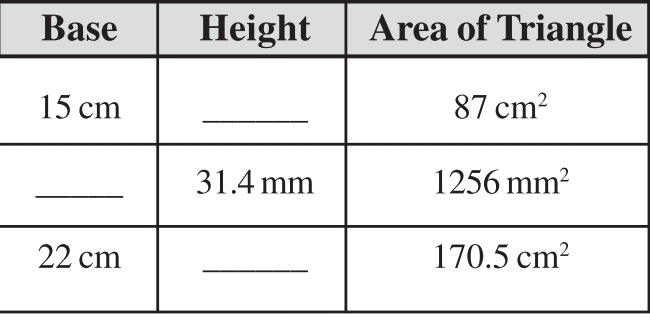
\includegraphics[width=\columnwidth]{figs/area1.jpg}
  \caption{}
  \label{fig:area1}
\end{figure}
\end{enumerate}
